\chapter{
Spatial capture-recapture models for partially identifiable populations/spatial mark-resight models
}
\markboth{Spatial mark-resight models}{}
\label{chapt.partialID}

\vspace{.3in}


So far, Chapters \ref{chapt.intro} �- \ref{chapt.XX} dealt with the situation where all detected individuals are identifiable, and in Chapter \ref{chapt.scr-unmarked} we introduced and developed an SCR model for non-identifiable populations, a spatial non-capture-recapture model, if you will. These two extremes are common in the study of animal populations with non-invasive sampling methods. However, there is also an intermediate situation, where a part of the population is tagged or otherwise marked and can thus be identified upon recapture, while the untagged portion remains unidentified. In this situation so-called mark-resight models XXXXX \citep{bartmann_etal:1987, arnason_etal:1991, neal_etal:1993}XXXX can be used to estimate population size and density combining data from both the marked and unmarked individuals. 
Mark-resight models have been around for a while (REFS). Traditionally, capture-recapture studies involve physical capture of individuals throughout the study; new individuals are marked on every re-capture occasion. In mark-resight, a sample of individuals is captured and tagged (or otherwise marked) during a single marking event that takes place prior to the resighting surveys. As such, mark-resight models have a major advantage over traditional capture-recapture models in that they only require individuals to be captured and handled once, during the initial marking. The resighting portion of the study can then be implemented using a non-invasive technique (hence the name �resighting�). This reduces field costs and risks for the animals (and potentially the researchers).

Mark-resight models have a set of underlying assumptions, most of which are analogous to those for mark-recapture models, e.g. demographic population closure (violation of geographic population closure can be accomodated by some models) and no loss or misidentification of marks. Just like regular capture-recapture models, there are means to incorporate temporal or individual heterogeneity in capture probability. However, a new and essential assumption of mark-resight models is that the tagged (or otherwise identifiable) individuals are a representative sample of the study population, so that inference about individual detection can be made for the whole population from the tagged sample. This issue is usually addressed by using a different method for marking than for resighting, and by marking a random sample of the population. For example, \citet{mace_etal:1994} tagged grizzly bears in XXX and then performed a camera-trap survey to estimate population size with mark-resight models. XXX MORE EXAMPLES XXX

\subsection{Types of partial ID data}
Before we start exploring mark-resight approaches in more detail, we need a clear understanding of what types of mark-resight data we can have, in order to appreciate and understand the different flavors of mark-resigh models. 
In general, we have (at least) two sets of data: encounter histories for identifiable individuals $i$ at trap $j$ and occasion $k$, $y_{ijk}$, and counts of unidentified records for each $j$ and $k$, $n_{jk}$. Depending on the sampling technique, we can conceive of three slightly different types of partial ID data. 

If you implement your resighting survey shortly after the marking session, you may be confident that none of the marked individuals has died or lost its marks. Under these circumstances you know that the number of marked individuals available for resighting, $m$, is equal to the number of individuals you tagged. Alternatively, tags might be radio-transmitters, allowing you to confirm the presence or absence of marked individuals in the resighting survey area using radio-telemetry \citep{white_shenk:2001}. In both cases, you know the number of marked individuals in the population you survey. 

In this situation, even though you may fail to resight some of the tagged individuals, since you know how many there are, you can simply assign them all-0 capture histories - in other words, contrary to regular capture-recapture models, in mark-resight models with a known number of tagged individuals, we can observe all-0 encounter histories. Under these circumstances, estimating $N$ reduces to estimating the number of unmarked individuals, $u$. 

A slight variation of this data type arises when in some instances we can only tell that an individual is tagged, but not who it is. You may be able to see that an individual is tagged but the identifying feature of the tag (maybe a number or coloration) may have become unreadable, or may be hidden from view. In this case, in addition to your $y_{ijk}$ and your $n_{jk}$ you also have a number of sightings of tagged but unidentified individuals, say $r_{jk}$.

If we suspect that some of the marks may have been lost between tagging and conducting the resighting samples, we obtain a slightly different type of mark-resight data. Here, we do not know the accurate number of marked individuals available for resighting. As a consequence, individuals have to be resighted at least once for us to know they are still tagged and alive and thus available for resighting. So, contrary to the situation where we know $m$ and analogous to regular capture-recapture models, we cannot observe all-0 encounter histories of marked individual. Here, estimating $N$ involves both estimating $m$ and $u$. 

A special case of this kind of data can arise from camera trapping. Even when dealing with a species that has no spots or stripes, some individuals in the study population can have natural marks that make them identifiable on pictures, such as scars or some distinct coloration. Again, in this scenario an individual has to be photographed at least once to be known. In case of camera-trapping, the fact that both the `marking� method and the subsequent resighting method are the same (although marking in this case does not involve any actual physical marking) can be cause for concern: our sample of `marked� individuals may not be a random sample of the population but consist of individuals that for some reason are more likely to be photographed. In that case, a basic assumption of the mark-resight model is violated.     

Finally, consider a scat or hair snare survey, where only a part of the samples are analyzed genetically (or DNA can only be extracted from a subset of samples due to sample quality). In this scenario, your $n_{jk}$ can contain both completely unknown individuals that are not represented at all in {\bf $Y$}, but it can also contain samples from individuals that we previously identified. The difference is that in the first two scenarios, part of the population of individuals is identifiable, while in the second scenario, part of the �population� of samples is identifiable. This type of data actually violates one of the basic assumptions of mark-resight models, namely, that tagged individuals are always correctly identified as such. To our knowledge there are currently no mark-resight models available that account for possible misidentification of individuals and in this chapter we will ignore this kind of data and focus instead on the two types of typical mark-resight data:  

\begin{itemize}
\item[(1)]	Known number of tagged individuals 
\item[(2)] Unknown number of tagged individuals, 
\end{itemize}


\subsection{An overview of mark-resight models}

Initially, mark-resight methods focused on radio-tagged individuals to estimate population size \citep{white_shenk:2001}. Radio-collars provide a means of determining which of the animals were in the study area and available for sampling, i.e. determining the number of marked individuals in the population. Knowing this number was a prerequisite for earlier mark-resight approaches. The oldest mark-resight model is the good old Lincoln-Petersen estimator, where individuals are marked and a single resight/recapture occasion is carried out \citep{krebs:1989}. We need not identify individuals, but only tell apart marked from unmarked individuals. Let $m$ be the number of marked individuals in the population, $m^{(R)}$ the number of marked individuals seen on the resighting occasion, and $n^{(R)}$ the total number of marked and unmarked individuals observed during resighting. Abundance $N$ is then estimated as 
\[
N = m \times n^{(R)}/m^{(R)}
\]

A suite of more elaborate models using individual capture histories over several resighting occasions were developed in the 1980ies and 90ies and compiled into the program NOREMARK \citep{white:1996}. Apart from the basic model with known number of marked individuals and no individual variation in resighting probabilities (joint hypergeometric maximum likelihood estimator) \citet{bartmann_etal:1987, white_garrott:1990, neal:1990, neal_etal:1993}, NOREMARK contains models that account for lack of geographical population closure \citep{neal_etal:1993}, individual heterogenenity in resighting rates and sampling with replacement (i.e. individuals can be seen more than once on any occasion, Minta and Mangel 1989, Bowden, 1993). A first mark-resight model allowing for an unknown number of marked individuals was developed by \citet{arnason_etal:1991}.

While many of these models perform well under certain situations, they are somewhat limited as they do not allow for combining data across several surveys \citep{mcclintock_etal:2006}. Also, not all of them are likelihood-based or allow for different parameterization, so that selection of the most appropriate model cannot be based on standard approaches such as AIC, but is largely left up to educated guesswork \citep{mcclintock_etal:2006}. Recently, more flexible and generalized likelihood-based mark-resight models have been developed. These models can account for individual heterogeneity in detection, unknown number of marked individuals and lack of geographical closure, as well as a less than 100\% individual identification rate of tagged individuals; they can be applied to sampling with and without replacement and can combine data across several primary sampling occasions in a robust design type of analysis \citep{mcclintock_etal:2009a,b, mcclintock_white:2009}. Since they are all likelihood-based, model selection among different parameterizations and model averaging based on AIC is an option. Most of these models have also been incorporated into the program MARK \citep{mcclintock_white:2010}.

Without going into much detail, these models are based on the joint likelihood of two major model components: one describing the resighting process of marked individuals (either using a Poisson or a Bernoulli observation model, depending on whether sampling is with or without replacement), where resighting probabilities can have both a fixed-effect and a random-effect component (on the appropriate logit or log scale) to accommodate variation in detection with time and due to individual heterogeneity, respectively; and one describing the total observations of unmarked individuals, $n_t$ which are approximated as a Normal distribution \citep{mcclintock_etal:2006}, or a Normal distribution left-truncated at 0 \citep{mcclintock_etal:2009}:
\[
n_t \sim Normal (E(n_t), V(n_t))
\]

In the simplest model case without any variation in detection, the expected number of resightings of unmarked individuals, $E(n_t)$, can be written as
\begin{equation}
E(n_t) = (N-m) * \theta 
\end{equation}
\label{partialID.eq.E_n}
where $\theta = k \times p$ for a Bernoulli observation model with $k$ replicas and individual detection probability $p$, or $\theta$ = individual encounter rate $\lambda$ for a Poisson observation model. The form of $V(n_t)$ depends on the underlying observation model, but like $E(n_t)$ it is based on the parameters that determine the individual detection probability/encounter rate. Using this formulation, $N$ is directly incorporated into the likelihood of the model.  
We see that while there are two likelihood components, they are both governed by the same parameters, which are informed by the data on marked individuals only. 
XXXXX go over the two McClintock papers and make sure I got this simplified description right XXXXX

In this chapter we will consider mark-resight sampling in the framework of spatial capture-recapture. We will look at models for both known and unknown numbers of marked individuals, and for imperfect individual identification of marks. In the spatial framework, most of the information on model parameters comes from the marked individuals. But in section \ref{} we will see that, analogous to the models we developed in the previous Chapt. \ref{}, the spatial correlation in counts of unmarked individuals also contributes information about detection and movement. 

\section{Spatial mark-resight model � known number of marked individuals}
Let�s begin with the traditional data situation: a known number of individuals constituting a random, representative sample from the population are marked and a series of resight samples are conducted following marking. All individuals are correctly identified as marked or unmarked, and marked individuals are 100 \% correctly identified to individual level. 
Under these conditions, the information obtained from the individually recognizable animals can easily be included into the spatial non-capture-recapture model we presented in Chapt. \ref{chapt.scr-unmarked}. Recall that without individual identity, the observed counts at trap $j$ and occasion $k$, $n_{jk}$, represent the sum of all latent individual detections at $j$ and $k$, $\displaystyle\sum\limits_{i=1}^{N}  y_{ijk}$, where $y_{ijk}$ are the latent individual encounter histories. We can model these counts as

\[
n_{jk} \sim \mbox{Poisson}( \Lambda_{j} )
\]


Under this formulation we do not need to update the individual $y_{ijk}$ in our model, which  is more efficient in terms of computing. However, we can also formulate the model as conditional on the latent $y_{ijk}$. This is useful because if we have $m$ individually known animals in our study population, than those $m$ $y_{ijk}$ are no longer latent, but fully observed and can easily be included in the analysis. 
The formulation conditional on $y_{ijk}$ basically brings us back to the original SCR model, where individual site and occasion specific counts, $y_{ijk}$, are modeled as
\[
y_{ijk} \sim \mbox{Poisson}(\lambda _{ij})
\] 
and
\[
\lambda _{ij} = \lambda_0 * exp(-D_{ij}^2/(2 \sigma^2))
\]

Unobserved $y_{ijk}$ are essentially missing data and have to be updated as part of the MCMC procedure. We can do that by using their full conditional distribution, which is multinomial with sample size $n_{jk}$:
\[
y_ujk \sim Multinomial (n_{jk}, \lambda_{uj})
\]
where {\bf u} is an index vector of the $M-m$ hypothetical unmarked individuals.
  
While in the non-spatial mark-resight analysis known individuals provide direct information about individual detection probability (or rate), in the spatial setting they also inform the movement parameter $\sigma$. Including known individuals into the analysis helps estimate model parameters more accurately and precisely. We will address the relationship between the number of marked individuals and accuracy of the estimated parameters in section \ref{sect.XX}. 

\subsection{MCMC for the spatial mark-resight model with known number of marked individuals}
Just as for the model without individual identification, for the partial ID model, knowing how to write your own MCMC algorithm comes in extremely handy. You will find that we only have to make relatively simple modifications to the MCMC code for the model without any individual identification presented in Chapt. \ref{chapt.scr-unmarked}, which, in turn, has much in common with the algorithms we developed for regular SCR models in Chapt. \ref{chapt.mcmc}. 

Essentially, we have to include an updating step for ${\bf Y}$, and modify the updating steps for $z_i$ and $\psi$ to reflect our knowledge of these parameters for the $m$ tagged individuals. 

First, we set up an array to hold ${\bf Y}$, fill the first $m$ rows of the array with the $m$ observed individual encounter histories, then update ${\bf Y}$ for the unknown individuals only:

\begin{verbatim}
# set up placeholders and create vectors for marked and unmarked    
 Y <- array(NA, c(M, J, K))
    nMarked <- nrow(y)
    marked <- rep(FALSE, M)
        marked[1:nMarked] <- TRUE
        Y[1:nMarked, , ] <- y
    z[marked] <- 1
    Ydata <- !is.na(Y)
    for (j in 1:J) {
        for (k in 1:K) {
            if (y[j, k] == 0) {
                Y[, j, k] <- 0
                next
            }
            unmarked <- !Ydata[, j, k]
            nUnknown <- n[j, k] - sum(Y[!unmarked, j,k])
            if (nUnknown < 0) 
                browser()
            probs <- lam[, j] * z
            probs <- probs[unmarked]
            probs <- probs/sum(probs)
                Y[unmarked, j, k] <- rmultinom(1, nUnknown, probs)
        }
    }
\end{verbatim}

When we knnow the number of marked individuals in the population estimating $N$ is reduced to etimating $u$. Thus, we only need to estimate the $z_i$ for $M-m$ unknown individuals (while we skip the update of $z_i$ for the �seen� individuals, seen is defined based on $Y$ and $Y$ is updated at each iteration, so the $z_i$ for the �seen� but unmarked individuals are effectively still updated). Thus, the updater for $z_i$ becomes:

\begin{verbatim}
       zUps <- 0
        seen <- apply(Y > 0, 1, any)
        for (i in 1:M) {
            if (seen[i] | marked[i]) 
                next
            zcand <- ifelse(z[i] == 0, 1, 0)
                ll <- sum(dpois(Y[i, , ], lam[i, ] * z[i], log = TRUE))
                llcand <- sum(dpois(Y[i, , ], lam[i, ] * zcand, 
                  log = TRUE))
            prior <- dbinom(z[i], 1, psi, log = TRUE)
            prior.cand <- dbinom(zcand, 1, psi, log = TRUE)
            if (runif(1) < exp((llcand + prior.cand) - (ll + 
                prior))) {
                z[i] <- zcand
                zUps <- zUps + 1
            }
        }
\end{verbatim}

Finally, this needs to be reflected in our update for $\psi$. In the full conditional beta distribution we have to replace $M$ with $M-m$ and $\sum z$ with $\sum z -m$:

\begin{verbatim}
  psi<-rbeta(1,1+sum(w[!marked]),1+sum(!marked)-sum(w[!marked]))   
\end{verbatim}

The remainder of the code is essentially identical to the MCMC code for regular SCR models we develped in Chapt. \ref{chapt.mcmc}.
You can find the full MCMC code (including the modeling options we'll discuss in the upcoming sections) in the accompanying {\bf R} package {\tt scrbook} by invoking {\tt scrPID()}. 

\subsection{Binomial encounter model}
XXX this section depends a little on whether we can work out the noID case XXXX
So far, we have only worked with Poisson encounter models for partially identifiable or unmarked populations. When we use a Bernoulli model instead, we have to make some changes to how we update the latent $y_{ijk}$, to ensure that a hypothetical individual receives at most a single observation at a given trap and occasion from the pool of $n_{jk}$ pictures. Effectively, we move from a multinomial situation where the same individual could be drawn repeatedly, to a sampling without replacement situation (an individual drawn once at $j$ and $k$ cannot be drawn again); here is how we implement this in our MCMC algorithm:

\begin{verbatim}
 Y <- array(NA, c(M, J, K))
#[...]
    for (j in 1:J) {
        for (k in 1:K) {
            if (y[j, k] == 0) {
                Y[, j, k] <- 0
                next
            }
            unmarked <- !Ydata[, j, k]
            nUnknown <- n[j, k] - sum(Y[!unmarked, j,k])
            if (nUnknown < 0) 
                browser()
            probs <- lam[, j] * z
            probs <- probs[unmarked]
            probs <- probs/sum(probs)
                Y[unmarked, j, k] <- 0
                guys <- sample(which(unmarked), nUnknown, prob = probs)
                Y[guys, j, k] <- 1
        }
    }
\end{verbatim}

\subsection{Example � Canada geese in North Carolina} 
We applied the spatial mark-resight model with a Bernoulli encounter model to a data set of Canada geese studied in North Carolina (Rutledge 2012). During the molting period of 2008, 751 individual geese were captured and tagged with neck and leg bands in XXXX, North Carolina. Geese were resighted at 87 different locations on 81 resightin events spread out over a period of almost two years. In addition to the banded geese, the number of unmarked geese was recorded during each resighting event. Here, we only looked at a subset of the data, from mid July to the end of October 2008, which corresponds to the first part of the post molt season, before migrating geese come back to the North Carolina breeding grounds.  
In this time block 746 of the 751 marked geese were known to be alive. Of those, 654 were resighted 3994 times at 40 different sites. In addition, 7944 sightings of unmarked geese were recorded at 48 sites. 
In this model, we also allowed $\sigma$ to vary between males and females. This only requires minor changes to the MCMC sampler and you can check these out by calling the XXX INCLUDE THAT?XXXX function from the {\tt scrbook} package.
We augmented the data set with 4500 - $m$ all-zero encounter histories, ran 50000 MCMC iterations and removed a burn-in of 1000 iterations. We provide all the data (data(canadageese)) and functions for you to repeat this analysis but be aware that given the large data set it will take days to do so. The model results, including the derived parameter density ($D$) are shown below. 
XXXX HAVE TO ASK FOR PERMISSION TO INCLUDE DATA XXXX

\begin{verbatim}
Iterations = 1001:50000
Thinning interval = 1 
Number of chains = 1 
Sample size per chain = 49000 

1. Empirical mean and standard deviation for each variable,
   plus standard error of the mean:

            Mean        SD  Naive SE Time-series SE
sigmaF    1.0594 1.902e-02 8.593e-05      0.0011674
sigmaM    1.1347 2.375e-02 1.073e-04      0.0014294
lam0      0.3245 8.037e-03 3.631e-05      0.0003103
psi       0.7924 3.284e-02 1.483e-04      0.0017778
phi       0.4337 1.857e-02 8.387e-05      0.0003754
N      3720.8128 1.210e+02 5.466e-01      6.6264003
D         6.6832 2.173e-01 9.817e-04      0.0119021

2. Quantiles for each variable:

            2.5%       25%       50%       75%     97.5%
sigmaF    1.0218    1.0470    1.0594    1.0717    1.0971
sigmaM    1.0909    1.1182    1.1341    1.1502    1.1834
lam0      0.3088    0.3191    0.3244    0.3298    0.3407
psi       0.7298    0.7698    0.7917    0.8143    0.8573
phi       0.3976    0.4210    0.4336    0.4462    0.4702
N      3492.0000 3637.0000 3717.0000 3802.0000 3961.0000
D         6.2722    6.5326    6.6763    6.8290    7.1146
\end{verbatim}

We see that credible intervals of estimates are pretty tight. Take, for example, $\sigma$ for males and females: Although they differ only by 0.08, there is barely any overlap between the respective credible intervals, surely an effect of the large data set.     




\subsection  {Individual identification rate of tagged animals <100 \%}
Often during resighting, it may be possible to see that an individual is tagged but impossible to determine the individual identity of the tag. In such a situation in addition to the $y_{ijk}$ and $n_{jk}$, we also have site and occasion specific counts of marked but unidentified individuals, $r_{jk}$. Here, the individual encounter histories of marked animals are essentially incomplete, and if we used these incomplete data to inform the detection parameter of the model, we would be likely to underestimate detection/trap encounter rate and overestimate abundance.
\citet{mclintock_etal:2009} suggest an intuitive means of correcting for this bias in a non-spatial model framework when dealing with a Poisson encounter model (or sampling with replacement). When marked but unknown resightings are part of the data, the expected value of $n_t$ changes from Eq. \ref{partialID.eq.E_n} to:

\[
E(n) = (N-m) { \lambda  + \eta/m}
\]
Here, $\lambda$ is the individual encounter rate estimated from the known resighted individuals and $\eta$ is the number of records of marked but unidentified individuals. So essentially, because $\lambda$ is known to be too low, the average number of unidentified pictures per known individual is added as a correction factor. This procedure assumes that the inability to identify a marked individual occurs at random throughout the population, which seems to be a reasonable assumption under most circumstances.

We can relatively easily translate this concept to our spatial mark-resight models.  In the spatial model framework we are interested in the individual and trap specific encounter rate, $lambda_{ij}$. Further, we do not look at the sum of all records of unmarked individuals, but formulate the model conditional on the latent individual encounter histories. Thus, instead of using $\eta/m$ as a correction factor, we need something that applies at the individual and trap level. If we take the sum of all correctly identified records of marked individuals, $\sum y_c$ and divide it by the total number of records of marked individuals, $\sum y_m$, we get the average rate of correct individual identification for marked individuals, say, $c$:
\[
c = \sum y_c/\sum y_m
\]

For the marked individuals we can then multiply $\lambda_0$ with $c$ to account for the fact that we observe incomplete individual encounter histories. For example, if on average we are able to assign 80\% of the records of marked animals to the correct individual, we would multiply $\lambda_0 \times 0.8$ for the marked individuals. Since we don't have this identification issue for unmarked individuals, their baseline trap encounter rate remains as before simply $\lambda_0$ (or in other words, their $c$ equals 1). Observe that now, in addition to assuming that failure to identify tagged individuals occurs at random throughout the population, we also assume that it occurs at random throughout space, i.e. our success of identifying a tagged individual does not depend on the trap we encounter it in. 
It is straightforward to  include this correction factor in our MCMC algorithm, by simply specifying a vector of length $M$, where $c = 1$ for all unmarked (hypothetical) individuals and $c = \sum y_c/\sum y_m$ for all marked individuals. Incomplete individual identification of marked individuals is included as an option in the {\tt scrPID} function.

XXXX maybe we can include the ISSJ as an example XXX

\section {Spatial mark-resight models for unknown numbers of marked individuals}

Now let us consider the case where we do not know the exact number of tagged individuals available for resighting so that we have to capture an individual at least once to be sure that it is available. As a consequence, we cannot observe all-0 encounter histories for the marked individuals. When using maximum likelihood inference, this situation requires a model where detection rates of known individuals are modeled using a zero-truncated distribution \citep{mcclintoc_etal:2009}. If we did not account for the fact that 0�s are unobservable, our estimates of detection rates would be artificially inflated and estimates of population size would be negatively biased. 

Working with zero-truncated distributions in a spatial mark-resight setting is less straight-forward than for non-spatial mark-resight. A marked individual only has to show up once, anywhere on the sampling grid, for us to know that it is there. When resightings are pooled across the entire sampling grid,then the total individual counts $\sum_j y_{ij}$ have to be >0 for all resighted individuals and a zero-truncated distribution can be used to model these counts. However, we are concerned with trap-specific encounters, $y_{ij}$, which can easily be 0 for a resighted individual, as long as a single $y_{ij}$ is > 0. Thus, the zero-truncation does not apply to the individual and trap specific counts we observe, but only to the sum of these counts over all traps. 

As an alternative to a zero-truncated distribution, in a Bayesian framwork, we can make use of data augmentation to estimate the number of marked individuals\footnote{for the interested reader, \citet{mcclintock_hoetig:2010} implement a non-spatial mark-resight model with a binomial observation model in a Bayesian framework using data augmentation}. 
In the previous example, where we knew the number of marked individuals, we essentially removed those individuals from the augmented population by fixing their $z_i$ at 1 and letting $\psi$ refer only to the unmarked population, $M-m$. All we have to do in the spatial mark-resight model with unknown number of marked individuals is to let our marked individuals be part of the augmented population again, analogous to the situation in regular SCR models:
\begin{verbatim}
        psi <- rbeta(1, 1 + sum(z), 1 + M - sum(z))
\end{verbatim}
Again, an unknown number of marked individuals is included as an option in {\tt scrPID}, and the options of incomplete individual identification of marks as well as both observation models apply to this sampling situation, too.
 
XXXX Other example data set? XXXX
XXXX Alternatively, I could include some simulated data sets with the model descriptions and put the real life example (geese) here at the end XXXXXXXXXX

\section{How much information do marked and unmarked guys contribute?}
To evaluate how adding marked individuals to a population improves parameter esimtates over a sampling situation without any identifiable individuals, we performed a small simulation study.  We used a 15 � 15 trap grid and
simulated detection data of $N = 75$ individuals in a 20 x 20 units state-space over $k = 5$ occasions with
$\sigma = 0.5$, $\lambda_0 = 0.5$. We generated 100 datasets each for
$m$ = (0, 5, 15, 25, 35) where $m$ is the number of marked individuals randomly sampled from the population.

Without any marked individuals in the population, posterior distribution of $N$ is fairly skewed, but its mode is still an approximately unbiased point estimator of $N$. As anticipated, posterior precision increases substantially with the proportion of marked individuals (Tab. \ref{partialID.tab.sim} and Fig. \ref{partialID.fig.nposts}). The posterior mode was approximately unbiased as a point estimator, and the root-mean squared error decreased from 19.076 when all 75 individuals were unmarked to 6.398 when 35 individuals were marked (Tab. \ref{partialID.tab.sim}). Coverage was nominal for all values of $m$ and posterior skew was greatly diminished (Tab. \ref{partialID.tab.sim}).

\begin{figure}[ht]
  \centering
  \includegraphics[width=4in,height=4in]{Nposts2.eps} % was 3,7
  \caption{Overlaid posterior distributions of $N$ from 100 simulations
    for four levels of marked individuals.}
  \label{partialID.fig.nposts}
\end{figure}

\begin{table}[hb]
\caption{Posterior mean, mode, and associated RMSE for simulations in
  which $m$ of $N$=75
  individuals were marked. One hundred simulations of each case were
  conducted. }
\begin{tabular}{lrrrrr}
      & Mean   & RMSE   & Mode   & RMSE   & Coverage \\
\hline
 m=0  & 85.866 & 24.735 & 77.660 & 19.076 &  0.940 \\
 m=5  & 80.096 & 13.948 & 76.270 & 13.635 &  0.980 \\
 m=15 & 78.763 & 11.548 & 76.110 & 10.964 &  0.940 \\
 m=25 & 77.658 &  8.826 & 75.810 &  8.562 &  0.950 \\
 m=35 & 76.385 &  6.453 & 74.900 &  6.398 &  1.000 \\
\hline
\end{tabular}
\label{partialID.tab.sim}
\end{table}

% \section{ SCR models for a partially identifiable �population of samples�}
% If we can figure that out�

\section{summary}
